\section{Giới thiệu. Ghi chú}

%% For our purposes here, ``theorems'' are labelled enunciations,
%% often set off from the main text by extra space and a font change.
%% Theorems, corollaries, conjectures, definitions, examples, 
%% remarks, and proofs are all instances of ``theorems''.  
%% The ``header'' of 
%% these structures is composed of the type of the structure 
%% (such as \textsc{Theorem} or \textsc{Remark}), a number 
%% which serializes the instances of the same type throughout the
%% document, and an optional name (such as ``Correctness Theorem'').
Một môi trường tựa định lý, ta gọi tắt là |THM|, được minh họa
như ở Hình~\ref{fig:THM}. Với mỗi |THM|, các tên |định lý|, |hệ quả|, |bổ đề|, |tiên đề|,
|định nghĩa|, |ví dụ|, |ghi chú|, |chứng minh|,\ldots
được gọi là \emph{tên của} |THM|.
Phần |header| của |THM| bao gồm tên của |THM|, chỉ số của |THM|,
tên tuỳ chọn (hay tên riêng) của |THM|. Phần nội dung của |THM|
còn gọi là \emph{thân} của |THM|. Để ý rằng, tên của |THM| khác
với tên của môi trường |THM|.\footnote{Trong thực tế, thường tên
của môi trường \texttt{THM} và tên của \texttt{THM} có sự tương ứng
1-1, ví dụ \texttt{menhde} ứng với \texttt{Mệnh đề},
\texttt{dinhly} ứng với \texttt{Định lý}. Do đó, trong đa số trường hợp,
sự phân biệt này không có ý nghĩa quan trọng\ldots --- kyanh}
Trong ví dụ sau,
\begin{example}
  \newtheorem{foobar}{Menh de}
\end{example}
ta có |THM| với tên là |Menh de|, nhưng tên của môi trường
tương ứng là |foobar|. Đôi khi, ta sẽ gọi \emph{môi trường} |THM| thay cho
\emph{tên của môi trường} |THM|.
%% dùng để chỉ loại của cấu trúc (ví dụ định lý hay
%% định nghĩa), chỉ số của cấu trúc và tên tuỳ chọn (ví dụ |Tiên đề chọn|).
%% Các (tựa) định lý thường phải được trình bày rõ ràng, tách biệt
%% với các phần khác cùa tài liệu, bằng cách thêm các khoảng trắng
%% thích hợp, thay đổi kiểu chữ. 

%% The layout of theorems can be changed by parameters as the fonts
%% of the header and the body, the way how to arrange the headers,
%% the indentation, and the way of numbering it.
%% Confronted with these requirements, |theorem.sty|, a style for 
%% dealing with theorem layout was developed by Frank Mittelbach
%% which was the standard theorem-environment for long time.
\medskip
Cách thể hiện |THM| có thể được thay đổi nhờ các tham số về
kiểu chữ cho |header|, cho thân |THM|, các bố trí |header|, khoảng trắng
thụt đầu dòng, cách đánh số,\ldots Để thỏa mãn các yêu cầu thay đổi này,
gói |theorem.sty| của Fran Mittelbach đã được viết và trở thành
gói chuẩn của \LaTeX{} từ rất lâu.

%% But then the desire for additional features like ``endmarks''
%% and ``theorem-lists'' arose. 
%% Two extensions of |theorem.sty| were developped: One for handling 
%% endmarks, |thmmarks.sty| and one for generating lists, |newthm.sty|. 
%% Thus, Frank Mittelbach suggested to combine the new features into 
%% one ``standard-to-be'' package. 
%% And now, here it is.
\medskip
Tuy nhiên, các tính năng khác nhưng dấu kết thúc |endmarks|, danh sách
các |theorem| vẫn chưa được hỗ trợ bởi gói chuẩn đó. Giải quyết vấn đề này,
có hai mở rộng của gói |theorem.sty| được phát triển: một gói chuyên về
điều khiển |endmarks|, gói |thmmarks.sty|, và một gói chuyên về liệt
kê danh sách |THM|, gói |newthm.sty|. Sau đó, Frank Mittelbach đề nghị
kết hợp các hỗ trợ của hai gói này vào cùng một gói mới (sẽ là chuẩn).
Đó chính là gói |ntheorem.sty| ;)

\begin{figure}[bht]
\begin{center}
	\ifpdf
		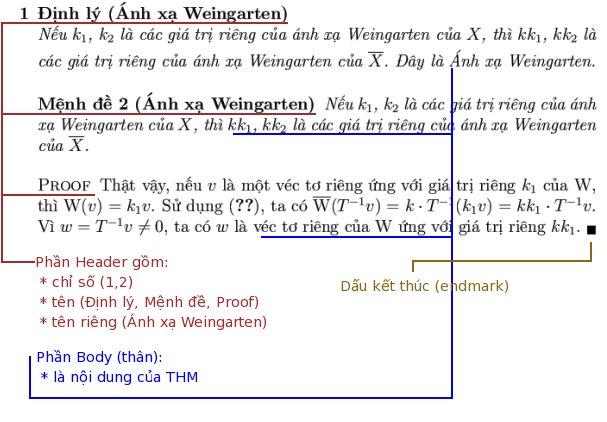
\includegraphics[scale=.6]{thm.png}
	\else
		\includegraphics[scale=.6]{thm.ps}
	\fi
\end{center}
\caption{Môi trường THM}
\label{fig:THM}
\end{figure}

\endinput
